\chapter{Sensor Networks}
In this chapter we begin with an introduction to wireless sensor networks (WSNs), compare them briefly to RFID systems, and then move into applications and a practical MAC protocol used by many wireless systems (CSMA/CA).

An RFID system and a wireless sensor network might look similar at first glance because both involve small wireless devices dispersed in an area. But they have very different roles and capabilities.
\begin{itemize}
    \item An RFID deployment is usually built around a reader that interrogates inexpensive passive or active tags. The tags typically send an identifier only. The communication topology is usually a star: the reader sits in the center and tags respond when interrogated.
    \item In sensor networks, a \textit{sensor node} is more like a small computer with a radio, a microcontroller, some sensors, storage and a battery. Unlike passive RFID tags, sensor nodes can continuously sense environmental data, perform local computation, schedule transmissions, and run networking protocols (see Figure \ref{fig:sensor-network1}). Many sensor networks are multi‑hop: data can hop from node to node until it reaches a sink or gateway that aggregates data and forwards it to servers on the Internet.
\end{itemize}

\begin{figure}[ht]
    \centering
    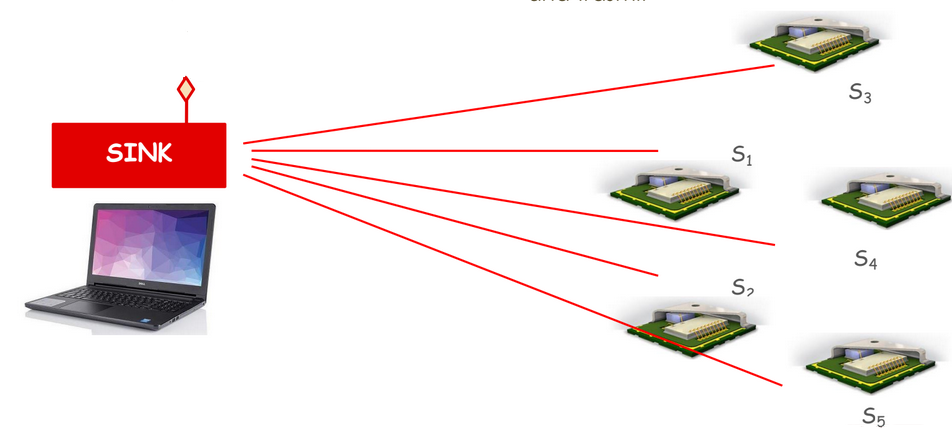
\includegraphics[width=0.8\linewidth]{images/sensor-network1.png}
    \caption{Sensor network.}
    \label{fig:sensor-network1}
\end{figure}

\section{Wireless Sensor Networks}
A sensor node is composed of of several components: a sensor to measure some physical quantity, an antenna and radio transceiver for wireless communication, a processor to run local code and coordinate sensing and communication, a battery that supplies power, and an optional flash memory for local logging.

A common architecture in WSN deployments goes like this. Each node senses the monitored area and periodically sends measurements to a sink node. The sink collects and may pre‑process the data; often it is connected to a server and the Internet so the data can be stored, analyzed or shown on user dashboards (see Figure \ref{fig:sensor-networks}).

There are three main benefits that explain why industries and researchers are so interested in WSNs.
\begin{itemize}
    \item \textit{Scale:} sensor networks let you cover large geographic areas, even in remote or inaccessible locations. 
    \item \textit{Autonomy:} once installed, they can run autonomously for long stretches, reducing the need for human intervantion. 
    \item \textit{Timeliness:} because many applications require fast reaction, WSNs provide near real‑time data and can trigger automated responses.
\end{itemize}

\subsection{Applications of Wireless Sensor Networks}
If a physical space needs monitoring or if a process would benefit from distributed sensing and feedback, a WSN can help. We'll now list the many application areas where WSNs are used.
\begin{itemize}
    \item \textit{Environmental monitoring and agriculture.} Sensor networks can measure temperature, humidity, light, rainfall, river levels and ground vibrations. A typical use case is using distributed sensors in a forest to detect early signs of wildfire, because local increases in temperature and changes in humidity can indicate conditions favorable to fire. In agriculture, sensors can measure soil moisture and temperature, allowing irrigation systems to water only where and when it is needed. This saves water and improves yield.
    \item \textit{Structural Health Monitoring (SHM).} SHM uses sensors to observe changes in a structure’s material or geometry over time. The goal is to detect deterioration or damage early and avoid costly failures. SHM is relevant during construction, right after an impact or shock, and much later in a structure’s life as it ages. Wireless sensor networks allow non‑intrusive monitoring, often at a lower cost than wired solutions.
    \item \textit{Health care and assisted living.} Sensors on or around people can track vital signs, movement, and activity to support rehabilitation programs, chronic disease management, or fall detection for elderly people living at home. Wearables like accelerometers and heart rate monitors can feed data to personal devices and cloud services to provide personalized wellness guidance.
    \item \textit{Marine and underwater monitoring.} Placing sensors in the ocean gives us a way to map the seafloor, monitor ecosystems, or watch for pollution. Underwater wireless networks are their own subdiscipline because radio doesn’t propagate well underwater — acoustic communications or special underwater optical links are often used instead.
\end{itemize}

\subsection{Characteristics of WSN}
In any WSN three logical roles appear repeatedly: sources, sinks, and actors. 
\begin{itemize}
    \item A \textit{source} is a sensor node that measures environmental data and reports those measurements somewhere. 
    \item A \textit{sink} is the entity that wants to receive the data for storage, display, or analysis. 
    \item An \textit{actors} (also called actuators) react to data: they control actuators or devices when certain conditions are met, enabling closed loops between sensing and action.
\end{itemize}

How you place nodes depends on the scenario.
\begin{itemize}
    \item When a site is inaccessible or when deployment must be quick, nodes can be dropped from an aircraft. This yields a roughly uniform random distribution across a finite area and is common in disaster response or environmental monitoring.
    \item When predictability and coverage guarantees matter, nodes are deployed in a planned, regular fashion. Regular placement is convenient in bridges, buildings, or industrial settings where you can attach sensors at pre‑decided locations to monitor critical spots.
    \item Nodes can also be mobile. Mobility may be passive — a sensor drifting with water currents — or active — a robot or drone moving purposefully to improve coverage or gather data from interesting areas. Mobile nodes can help compensate for random deployment shortcomings, can reposition themselves in response to events, or can be used as collectors of data from stationary nodes.
\end{itemize}
At the hardware level a sensor node combines sensing, processing and networking on a small board (see Figure \ref{fig:sensor-node-components}). The primary components are:
\begin{itemize}
    \item An RF transceiver and antenna to send and receive wireless packets; 
    \item A microcontroller or CPU to run software, perform preprocessing, and coordinate the node; 
    \item A memory and flash storage to buffer and log data; 
    \item A sensing unit composed of one or more transducers (temperature, humidity, accelerometer, etc.); 
    \item A power source, usually a battery or energy harvester.
\end{itemize}
These pieces work together: the sensor reads analog values, a conditioning circuit cleans and scales the signal, an ADC converts it to digital, the CPU may compress or aggregate the reading, and the transceiver sends packets to neighbors or to a sink. Because power is precious, these functions are often duty‑cycled: sensors and radios sleep much of the time and wake up briefly to sample or transmit.

\begin{figure}[ht]
    \centering
    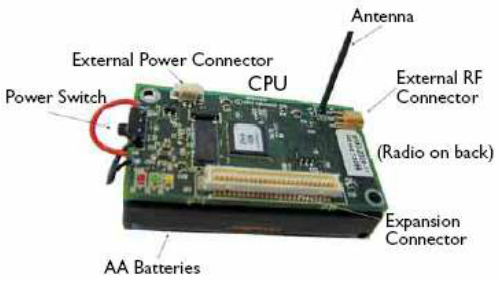
\includegraphics[width=0.5\linewidth]{images/sensor-node-components.png}
    \caption{Sensor node components.}
    \label{fig:sensor-node-components}
\end{figure}

Embedded operating systems are common on sensor nodes to simplify programming and concurrency. TinyOS is a lightweight OS originally developed at UC Berkeley specifically for devices with strict resource constraints. TinyOS is written in and programmed using NesC, a dialect of C designed for component‑based, event‑driven programming.

A few practical constraints dominate WSN design.
\begin{itemize}
    \item WSNs are expected to scale. A good design should support a large number of nodes without the system collapsing under its own signaling overhead. At the same time, the same design should work for small installations. So the protocols and algorithms used in WSNs must perform well across a wide range of node densities and deployment sizes.
    \item Nodes must be cheap, small, and energy-lean. Because they’re usually battery powered, energy is the resource engineers worry about first. 
    \item Memory and processing power are modest, radios are simple, and sometimes nodes don’t even have a global address like an IP. 
    \item Topologies can be mostly static, but there are growing deployments where node roles or positions change continuously — for example when mobile robots are used.
    \item Quality-of-service concepts familiar from classical networks need to be reinterpreted. Traditional metrics like throughput or latency still matter in some applications, but other concerns — energy efficiency, robustness to node failure, graceful degradation — are often more important. 
    \item A sensor network should keep delivering the services it was designed for as long as possible; how “long” is defined by the application. Sometimes the goal is to maximize the lifetime of the whole network (e.g., keep the area monitored), while in other cases the lifetime of individual nodes matters less than preserving coverage or connectivity.
    \item Robustness is essential. Nodes can fail because they run out of battery, get damaged, or lose connectivity. The network should tolerate such failures and adapt: routes should reroute around dead nodes, and the system should be able to incorporate newly deployed nodes.
    \item Reprogramming nodes after deployment is often necessary — for bug fixes, configuration changes, or to change sensing behavior. 
    \item Maintainability also includes the ability to self-monitor and adapt configuration at runtime. The network should be able to change duty cycles, adjust sensing schedules, or reassign roles to match changing conditions.
    \item A handful of mechanisms show up again and again because they address the key constraints of sensor networks. Multi-hop wireless communication is used to extend range and conserve energy by allowing nodes to forward packets for each other. 
    \item Energy efficiency is pursued at every layer. Communication protocols minimize transmissions, computation is used to reduce transmitted data, and sensing schedules avoid wasteful sampling.
    \item Data-centric networking means designing around the information the network must provide rather than around node identifiers. 
    \item Locality means do as much as possible locally — on a node or among its close neighbors — because local communication is cheaper than long hops.
\end{itemize}
Sensor networks exist to let us collect information from the physical world even in places that are hard to reach, to directly couple human decision-makers and automated systems to those measurements, and to provide information with precise spatial and temporal localization.

\subsection{Wireless signal}
Wireless communication is fundamentally different from wired because the radio signal weakens and distorts as it travels through space. Signal strength decreases with distance: energy is spread over a larger area as the wavefront expands, and in real environments obstacles cause additional loss. This attenuation is why range is limited and why placement and power settings matter.

When discussing ranges in wireless communications we commonly refer to three related concepts. 
\begin{enumerate}
    \item The \textit{transmission range} is the distance over which the sender’s signal is strong enough that the intended receiver can decode it under typical conditions. 
    \item The \textit{detection range} is the distance at which the receiver can detect that something is being transmitted but the signal may be too weak or noisy to decode correctly. 
    \item The \textit{interference range} can be even larger: a transmitter far away may not be heard reliably, but its transmissions can still raise the noise floor at a receiver and disrupt reception of other nearby transmitters.
\end{enumerate}
Real environments introduce multipath (see Figure \ref{fig:multipath-wireless-signal}): when radio waves encounters an obstacle, all or part of the wave is reflected, with a loss of power. A source signal can be reflected and multiple copies may arrive at the receiver at different times and phases. These multiple paths can add constructively or destructively, causing fading, delay spread, and intersymbol interference.

\begin{figure}[ht]
    \centering
    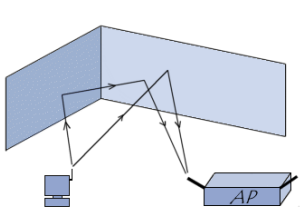
\includegraphics[width=0.4\linewidth]{images/multipath-wireless-signal.png}
    \caption{Multipath wireless signal.}
    \label{fig:multipath-wireless-signal}
\end{figure}

Interference arises both from multipath of the same sender and from other transmitters using the same frequency band. A receiver might receive several overlapping signals, and if they overlap in time and frequency they can corrupt each other. The signal-to-noise ratio (SNR) captures the the ratio of good to bad signal. High SNR means the signal is stronger than the noise and the receiver has a good chance of decoding the data; low SNR means that the signal has been damaged by noise and errors are likely.

\subsubsection{Hidden and Exposed Terminal Problems}\label{sec:hidden-and-exposed-terminal-problems}
Two classic problems make medium access control in wireless networks interesting and often tricky: the hidden terminal problem and the exposed terminal problem.

Imagine three nodes labeled \texttt{A}, \texttt{B}, and \texttt{C}. \texttt{A} and \texttt{C} are out of range of each other, but both can reach \texttt{B}. If \texttt{A} wants to send to \texttt{B} and \texttt{C} also wants to send to \texttt{B}, \texttt{A} and \texttt{C} cannot sense each other’s transmissions (they are “hidden” from each other), so they may transmit simultaneously. At \texttt{B} those concurrent transmissions collide and both packets are lost. The problem is “hidden” because \texttt{A} doesn’t know about \texttt{C} and vice versa even though their simultaneous transmissions interfere at the receiver (see Figure \ref{fig:hidden-terminal-problem}).

\begin{figure}[ht]
    \centering
    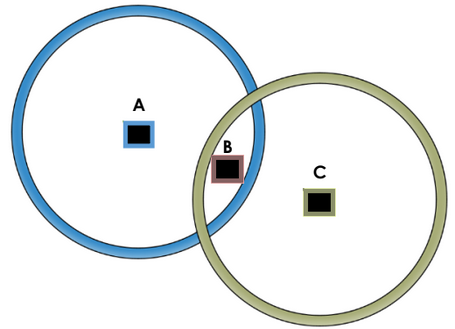
\includegraphics[width=0.45\linewidth]{images/hidden-terminal-problem.png}
    \caption{Hidden terminal problem.}
    \label{fig:hidden-terminal-problem}
\end{figure}

Now imagine a different scenario. Suppose \texttt{B} is transmitting to \texttt{A}, and \texttt{C} is nearby the sender \texttt{B} but wants to transmit to \texttt{D}, which is out of range of \texttt{B} but within range of \texttt{C} (see Figure \ref{fig:exposed-terminal-problem}). If \texttt{C} senses \texttt{B}’s transmission, it may refrain from sending because the medium appears busy. However, \texttt{C}’s transmission to \texttt{D} might not interfere with \texttt{B}’s reception at \texttt{A}, so the silence is unnecessary and hurts channel utilization. \texttt{C} is “exposed” to \texttt{B}’s transmission and is being overly conservative.

\begin{figure}[ht]
    \centering
    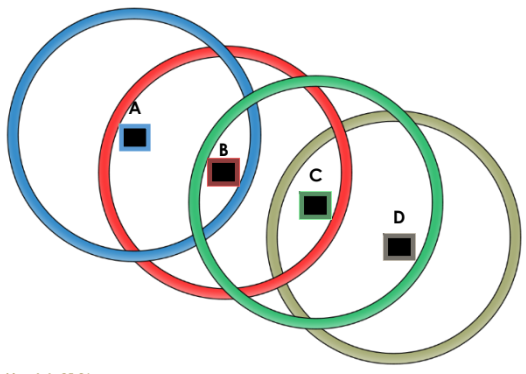
\includegraphics[width=0.55\linewidth]{images/exposed-terminal-problem.png}
    \caption{Exposed terminal problem.}
    \label{fig:exposed-terminal-problem}
\end{figure}

Those two problems pull MAC design in opposite directions: you want to avoid collisions caused by hidden terminals, but you also don’t want to unnecessarily silence nodes that could transmit safely.

\section{Medium Access Control (MAC)}
Medium Access Control — MAC for short — is the part of a wireless system that controls when a node should transmit and when it should listen. Those two operations — sending and listening — are arguably the most important operations for any wireless device, because they directly drive energy use and the user-visible performance of the system. Listening with the radio powered on, waiting idly for packets that may never arrive, can consume as much energy as a short transmission. So MAC design tries to:
\begin{itemize}
    \item prevent collisions and therefore reduce retransmissions,
    \item be energy efficient, especially by avoiding unnecessary idle listening,
    \item scale: a scheme that works for ten nodes but collapses at a hundred is not suitable for many WSN applications,
    \item meet latency requirements when they exist, 
    \item be fair to nodes that need to transmit, 
    \item use bandwidth efficiently,
    \item provide reasonable throughput.
\end{itemize}
In sensor networks, energy efficiency and collision avoidance often sit higher on the priority list than raw throughput.

Sensor nodes usually run from batteries. In many deployments swapping or recharging batteries is expensive, dangerous, or impossible. Because the battery capacity is finite, every design decision that affects how much time a node’s radio or CPU spends active also affects the system’s lifetime.

Nodes are often idle most of the time and wake only when something interesting happens, when they need to forward data, or on a periodic schedule. That sporadic activity pattern means the MAC must be tuned to avoid wasting energy during the long idle stretches while still providing timely delivery when activity happens.
There are a handful of recurring ways energy is lost in WSNs:
\begin{itemize}
    \item \textit{Collisions} happen when two or more transmissions overlap at a receiver. When packets collide they are usually corrupted and must be retransmitted. Retransmissions cost both sender and receiver energy and increase network congestion.
    \item \textit{Overhearing} happens when a node receives a packet intended for somebody else. Radios on nearby nodes will pick up transmissions they don’t need, expend energy to receive and process headers, then discard them.
    \item \textit{Control-packet overhead} includes the handshakes, beacons, periodic sync messages and other small packets that support the protocol. Too many control packets can offset the savings from reduced collisions or improved coordination.
    \item \textit{Idle listening} is when the radio is powered and waiting for traffic that never arrives. Because listening power is non-negligible, long periods of idle listening quickly drain battery.
    \item \textit{Overemitting} is wasted transmit energy when a sender transmits while the intended receiver is not ready — for example the receiver is asleep or out of range.
\end{itemize}

\subsection{MAC protocols}
Different applications induce different traffic patterns:
\begin{itemize}
    \item One common pattern is broadcast or interest dissemination, where the sink or base station transmits a message intended for all nodes. This happens when a controller wants to query the network, push a configuration change, or distribute a code update.
    \item The other common pattern is convergecast or data gathering: many sensors send observations up to a single sink. This is asymmetric traffic (many-to-one) that can be used for collection of data from the environment or sensor network management and monitoring.
\end{itemize}
To design a good MAC protocol for wireless sensor networks, the following attributes must be considered:
\begin{itemize}
    \item \textit{Energy efficient.} It must conserve energy to extend network lifetime, yet adapt to changes in node density and topology. 
    \item \textit{Scalability and adaptability.} Protocols should behave sensibly from small testbeds to large-scale deployments.
    \item \textit{Latency, throughput and bandwidth utilization} are important too, but many sensor applications can tolerate higher latency in exchange for longer node lifetimes.
\end{itemize}
At a high level MACs fall into two families: contention-based and schedule-based.
\begin{itemize}
    \item \textit{Contention-based} protocols allocate the channel on demand. Nodes that have data to send first sense the channel to check whether it’s free; if it is, they transmit, often using randomized backoffs to reduce the chance that two nodes transmit at once. This approach is decentralized, scales without a central controller, and adapts dynamically to traffic, which makes it attractive in ad hoc and highly variable environments. But contention-based MACs suffer from idle listening, collisions, and interference; as node density increases, the probability of collision grows and energy costs can climb.
    \item \textit{Schedule-based} protocols assign explicit times when each node may transmit. The schedule can be fixed or generated on demand, and when it is enforced collisions are essentially eliminated, which saves retransmissions and energy. They tend to be more energy-efficient in steady-state, because nodes know exactly when to wake and when to sleep. However, schedules require synchronization and some form of centralized coordination or distributed agreement to create the schedule, and that overhead can be costly.
\end{itemize}
Sensor networks often use hybrids: schedules for predictable periodic reporting, combined with contention-based access for bursty or event-driven traffic. Many modern MACs adaptively change behavior depending on load.

\subsection{CSMA/CA}
\textit{Contention-based MAC} (Medium Access Control) protocols are the polite, distributed rules that let many wireless stations share the same radio channel without a brawl. The most widely used of these rules in Wi-Fi is called \textit{CSMA/CA — Carrier Sense Multiple Access with Collision Avoidance}.

In wired Ethernet you can often detect a collision while you’re transmitting: the voltage on the wire betrays that something else has transmitted at the same time, and you stop and retry. Wireless is not so forgiving. When a station transmits over the air it typically cannot listen at the same time and reliably measure whether its signal collided with someone else’s. Because collisions are hard to detect, the philosophy shifts from collision detection to collision avoidance.

In CSMA/CA, when a station has a packet to send it
\begin{enumerate}
    \item Listens to the channel. 
    \item If the channel is idle, the station waits a short fixed gap called an inter-frame space (IFS). If the channel remains idle for this IFS interval, the station may start transmitting immediately. 
    \item If the channel is busy when the station senses it, or it becomes busy during that IFS waiting period, the station defers transmission. It keeps monitoring the channel until the current transmission ends.
    \item If the channel becomes idle again, the station does not necessarily transmit right away. Instead, to avoid many stations transmitting simultaneously after the channel frees up, each contending station enters a randomized backoff procedure: it chooses a random number of time slots from within a contention window and starts a backoff timer. That timer ticks down only while the channel remains idle. The first station whose backoff timer reaches zero takes the channel and transmits; others detect that transmission and freeze their timers, resuming them after the channel becomes idle again.
\end{enumerate}

\begin{figure}[ht]
    \centering
    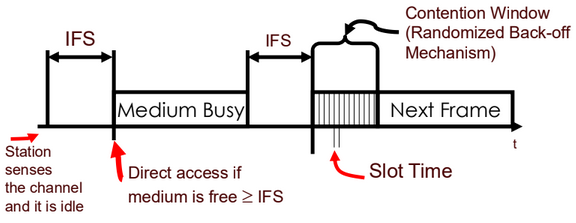
\includegraphics[width=0.7\linewidth]{images/basic-csma-ca.png}
    \caption{Basic CSMA/CA.}
    \label{fig:basic-csma-ca}
\end{figure}

Each station chooses a backoff counter uniformly at random between $[0, CW-1]$, where $CW$ is the current contention window size. The backoff is measured in slot times; the slot length depends on the physical layer, but conceptually a slot is the basic unit of "wait" in the protocol. All stations decrement their counters one slot at a time while the medium remains idle.

When the channel becomes busy before the counter reaches zero, the station freezes the backoff clock and waits for the next opportunity. Once the current transmission finishes and the channel has been idle for the required IFS, the station resumes decrementing the remaining backoff.

If a station’s packet collides or otherwise is not acknowledged, the protocol increases the contention window. In plain terms, the station becomes more conservative: it picks its next random backoff from a larger range, so that subsequent retries are less likely to conflict with others. This increase is exponential: after each failed attempt the station doubles the effective contention window (up to some maximum). That doubling is called \textit{binary exponential backoff}.

Not all transmissions are equal. Wi-Fi distinguishes priorities using different inter-frame spacing durations.
\begin{itemize}
    \item The shortest is SIFS, the Short Inter-Frame Space. SIFS is used for highest priority, very short control responses such as acknowledgments (ACKs), CTS (clear to send) messages, and other immediate replies. Because SIFS is shorter than the other IFS values, the recipient can reply quickly before others try to contend for the medium.
    \item PIFS, the point coordination function IFS, is a slightly longer gap used in schemes with a centralized controller; it sits between SIFS and DIFS in priority.
    \item DIFS, the distributed coordination function IFS, is the longest of the three basic values used by the DCF. Stations waiting to start a new asynchronous data transmission must see the channel idle for a DIFS interval before beginning their contention procedure.
\end{itemize}
This ordering SIFS $<$ PIFS $<$ DIFS ensures that short control replies (ACK, CTS) can be sent promptly and will not be preempted by ordinary data transmissions.

In the Distributed Coordination Function (DCF), an ordinary data transmission is followed by an acknowledgment from the receiver when the frame is correctly received (CRC check passes). The sender waits for DIFS before sending its data; the receiver, upon successful reception, responds after waiting only SIFS. Because SIFS is shorter than DIFS, the ACK from the receiver arrives before other stations opportunistically try to access the channel, preventing unnecessary retransmissions (see Figure \ref{fig:dcf-csma-ca-with-ack}).

If an ACK is not received in time, the sender assumes the frame was lost (either due to a collision at the receiver or a corrupted frame) and will schedule a retransmission following the backoff/retry rules.

\begin{figure}[ht]
    \centering
    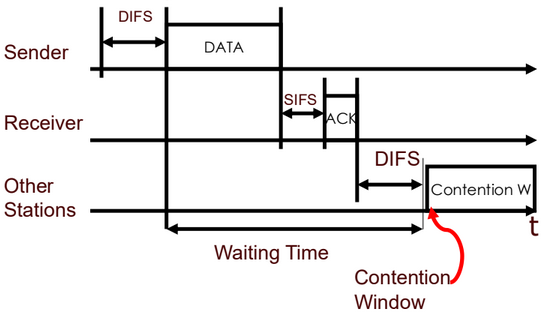
\includegraphics[width=0.65\linewidth]{images/dcf-csma-ca-with-ack.png}
    \caption{DCF CSMA/CA with ACK.}
    \label{fig:dcf-csma-ca-with-ack}
\end{figure}

\subsubsection{RTS/CTS}
To address hidden and exposed terminals, discussed in Section \ref{sec:hidden-and-exposed-terminal-problems}, 802.11 provides an optional reservation mechanism: Request-to-Send (RTS) and Clear-to-Send (CTS).
The sequence goes like this (see Figure \ref{fig:dcf-csma-ca-with-rts-cts}). 
\begin{enumerate}
    \item A station that wants to send data first senses the channel and, if idle for DIFS, transmits an RTS control frame to the intended receiver. The RTS contains, among other things, a duration field that indicates how long the impending exchange (RTS, CTS, DATA, ACK) will take.
    \item The receiver, if it hears and can accept the RTS, responds after SIFS with a CTS frame that echoes the duration. 
    \item Stations that hear either the RTS or the CTS set a timer called the Network Allocation Vector (NAV), which tells them how long the medium will be reserved. While the NAV is in effect those stations do not attempt transmissions, and so the sender can proceed to transmit the data packet without collision from those neighbors.
\end{enumerate}

\begin{figure}[ht]
    \centering
    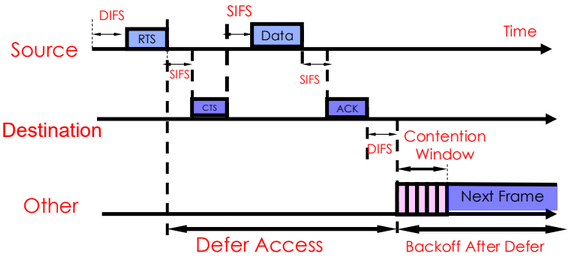
\includegraphics[width=0.7\linewidth]{images/dcf-csma-ca-with-rts-cts.png}
    \caption{DCF CSMA/CA with RTS/CTS.}
    \label{fig:dcf-csma-ca-with-rts-cts}
\end{figure}

RTS/CTS reserves the channel in two helpful ways. First, it lets the receiver tell nearby nodes to be quiet (solving hidden terminals). Second, it helps exposed terminals recognize situations where they are incorrectly deferring: a node that hears an RTS but then hears a CTS from a station that it cannot hear will interpret the medium differently and may proceed to transmit to its own neighbor if the NAVs indicate no conflict.

\begin{Example}{How RTS/CTS solves the hidden terminal problems}{}
Node \texttt{A} wants to send to \texttt{B} and sends an RTS. \texttt{B} responds with CTS. Node \texttt{C}, which could not hear \texttt{A} directly, will hear the CTS and thereby learn that \texttt{B} is about to receive from \texttt{A}. \texttt{C} sets its NAV and refrains from transmitting, preventing a collision at \texttt{B}.

\begin{minipage}{\textwidth}
    \centering
    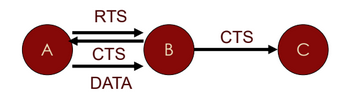
\includegraphics[width=0.5\linewidth]{images/rts-cts-hidden.png}
    %\captionsetup{hypcap=false}
    %\captionof{figure}{Query tree.}
    \label{fig:rts-cts-hidden}
\end{minipage}
\end{Example}
\begin{Example}{How RTS/CTS solves the exposed terminal problems}{}
Suppose \texttt{B} is sending to \texttt{A}. Node \texttt{C} hears \texttt{B}’s RTS to \texttt{A} and would normally defer. But if \texttt{C} examines the CTS and notices that it cannot interfere with the \texttt{A}–\texttt{B} exchange (for instance the NAVs and address fields indicate different receivers), \texttt{C} may be allowed to transmit to \texttt{D}.
\begin{minipage}{\textwidth}
    \centering
    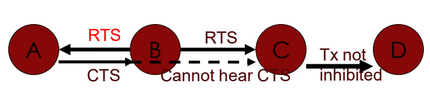
\includegraphics[width=0.6\linewidth]{images/rts-cts-exposed.png}
    %\captionsetup{hypcap=false}
    %\captionof{figure}{Query tree.}
    \label{fig:rts-cts-exposed}
\end{minipage}
\end{Example}

RTS/CTS reduces many collisions but does not eliminate them entirely. RTS frames themselves can collide if two nodes attempt RTS at the same time. Fortunately, since RTS frames are short, such collisions are less costly than data frame collisions. Stations whose RTS or data attempts collide follow the same exponential backoff scheme and retry. In short, the protocol accepts that collisions are inevitable on a shared, distributed medium and uses randomized backoff and retries to recover gracefully.

\subsubsection{Network Allocation Vector (NAV)}
Virtual carrier sensing is implemented in 802.11 by something called the Network Allocation Vector, or NAV. The NAV is essentially a local timer that a station sets when it hears a frame that says “I’m going to use the channel for $X$ more microseconds.” That duration tells the listeners how long the sender expects to occupy the medium for this exchange, including any immediate replies (think CTS, DATA, ACK and the short SIFS gaps between them). When a station transmits, it includes in that duration field the time required for its whole planned exchange. Any station that hears the frame and is not the intended recipient converts that duration into its own NAV timer and begins counting down.

While the NAV timer is greater than zero the channel is virtually busy. That means the station will not attempt to access the medium. When the NAV reaches zero, the station then checks the physical condition of the channel — if the PHY reports the medium is idle for the required inter-frame spacing, the station can start its contention procedure.

To see NAV in action, picture the complete RTS/CTS/DATA/ACK exchange (see Figure \ref{fig:nav}). 
\begin{enumerate}
    \item The sender first listens until the channel has been idle for DIFS; then it sends an RTS (Request to Send). That RTS includes a duration value that covers the time from the end of the RTS through the planned reply and data exchange.
    \item The receiver, after waiting only SIFS, replies with a CTS (Clear to Send). The CTS also contains a duration field: this is the remaining time of the planned exchange from the end of the CTS onward (the sender’s original duration minus the brief interval used by the RTS and CTS themselves). 
    \item Every station that hears either the RTS or the CTS sets its NAV based on those duration fields. Those stations then remain silent for that NAV period.
    \item Once CTS is received, the sender waits SIFS and then sends the DATA frame. The receiver, after SIFS, returns an ACK to confirm successful reception. When the ACK completes, the NAV reservations are effectively over and other stations may begin their own contention procedures.
\end{enumerate}

\begin{figure}[ht]
    \centering
    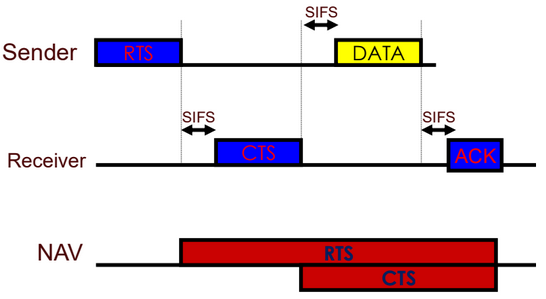
\includegraphics[width=0.7\linewidth]{images/nav.png}
    \caption{Network Allocation Vector (NAV).}
    \label{fig:nav}
\end{figure}

\subsection{S-MAC}
This section walks through S-MAC, a contention-based MAC protocol designed for wireless sensor networks (WSNs).

Wireless sensor nodes are often battery powered and expected to run for long periods without human intervention. Measurements show that idle listening can consume significant amount of energy, somewhere between 50\% and 100\% of the energy required for receiving.

Because a naïve CSMA/CA node keeps the radio on and keeps sensing the channel, that idle time adds up and wastes battery. There are other energy drains too: collisions that force retransmissions, overhearing (nodes receiving packets that are not for them), and control-packet overhead (the extra messages used to coordinate access). S-MAC’s core goal is to reduce those energy drains even if that comes at the cost of increased latency.

S-MAC asks nodes to be awake only when they need to be, and asleep for the rest. Nodes alternate between a listen period and a sleep period (see Figure \ref{fig:sleep-mac}). During sleep the radio is turned off completely and a the node sets a timer to awake itself lates, so it's not wasting power sensing the channel. When the node wakes up it listens for a while and either transmits, receives, or synchronizes with neighbors.

\begin{figure}[ht]
    \centering
    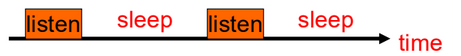
\includegraphics[width=0.6\linewidth]{images/sleep-mac.png}
    \caption{Sleep MAC.}
    \label{fig:sleep-mac}
\end{figure}

Each node adopts a repeating cycle: listen for a fixed interval, then sleep for a fixed interval, then listen again, and so on. Two terms are useful here:
\begin{itemize}
    \item \textit{Listen interval:} how long the node keeps its radio on in each cycle.
    \item \textit{Frame length (or cycle length):} the listen interval plus the sleep interval.
\end{itemize}
The duty cycle is the fraction of time the node’s radio is on. Mathematically,
\begin{equation*}
    duty\_cycle = \frac{listen\_interval}{listen\_interval + sleep\_interval}.
\end{equation*}

\begin{Example}{Duty cycle}{}
Reduce duty cycle to 10\% (listen for 200 ms and sleep for 2 s).

Let’s calculate that carefully. 
\begin{align*}
listen = 200ms\hspace{1cm}sleep = 2 s = 2000 ms\\
frame\_length = 200 ms + 2000 ms = 2200 ms\\
duty\_cycle = 200 / 2200 = 0.091 = 9.1\%\sim 10\%
\end{align*}
\end{Example}

\begin{Example}{Duty cycle}{}
If in each second a node sleeps for half a second and listens for the other half, duty cycle is 50\%.
\begin{align*}
listen = 0.5 s\hspace{1cm}sleep = 0.5 s\\
frame\_length = 0.5 + 0.5 = 1.0 s\\
duty\_cycle = 0.5 / 1.0 = 0.5 = 50\%
\end{align*}
\end{Example}

If everyone chose an independent listen/sleep schedule, what if a node wants to talk to another node that is sleeping? To avoid that, S-MAC groups neighbors into virtual clusters that share the same schedule. Neighbors who share schedules wake up and sleep at the same times; this keeps control overhead low and simplifies communication inside the cluster.

To achieve and maintain this alignment, S-MAC uses periodic synchronization messages called SYNC packets.
A SYNC packet is a short control message that tells to neighbors the sender’s next sleep time. It typically contains:
\begin{itemize}
    \item the sender’s node ID (so neighbors know who sent it),
    \item the next sleep time or the next wake time (a timestamp or relative offset that lets receivers align their local timers),
    \item sometimes other small metadata about the schedule.
\end{itemize}
There are two synchronization phases:
\begin{enumerate}
    \item \textit{Initial sync:} when a node first joins the network, it listens during its active period for SYNCs from neighbors. If it hears one, it adopts that schedule and becomes a \texttt{Follower}. If it hears none after a reasonable interval, it picks a schedule of its own and becomes a \texttt{Synchronizer} that announces that schedule.
    \item \textit{Periodic sync:} after synchronization is established, nodes continue to periodically send out SYNC packets to maintain synchronization, compensating for any clock drift that might occur over time.
\end{enumerate}
Each node keeps a small table of the schedules of its known neighbors (see Figure \ref{fig:schedule-tables}). Whenever a node receives a SYNC packet it records or updates the neighbor’s entry: who the neighbor is and when that neighbor will next be sleeping or listening. That table allows a node to know which neighbors it can expect to reach during a given active period.

\begin{figure}[ht]
    \centering
    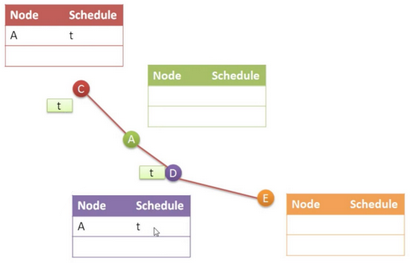
\includegraphics[width=0.6\linewidth]{images/schedule-tables.png}
    \caption{Schedule tables.}
    \label{fig:schedule-tables}
\end{figure}

When a node decides to set a schedule:
\begin{enumerate}
    \item First it listens to the medium for at least one synchronization period. 
    \item If it hears schedules from neighbors, it picks one of those schedules and becomes a \texttt{Follower}. \texttt{Followers} typically wait a random short delay and then re-broadcast the chosen schedule as a SYNC so neighbors know about it.
    \item If the node hears nothing during that initial listen window, it picks its own schedule and immediately broadcasts a SYNC saying “this is my schedule.” That node becomes a \texttt{Synchronizer} for nearby nodes.
    \item The random delay used by \texttt{Followers} before re-broadcasting helps prevent a flood of SYNCs at once, reducing collisions during the control window.
\end{enumerate}

Because different parts of a network may adopt different schedules, you end up with virtual clusters of nodes sharing a schedule. A node on the border between two clusters will hear and store schedule information from both clusters. That border node has a tricky role: when it needs to broadcast a packet that should reach nodes in both clusters, it may need to send multiple times — once timed to the first schedule and once timed to the other.

S-MAC is a contention-based protocol, which means that multiple neighbors who want to send to the same node will all try during that node’s listen window and must contend for the medium.

Before any transmission the node performs carrier sense: it listens to the channel to check whether someone else is transmitting. 
For unicast data, S-MAC follows the RTS/CTS/DATA/ACK handshake pattern (see Figure \ref{fig:dcf-csma-ca-with-rts-cts}). The sender first sends a Request To Send (RTS). If the intended receiver hears it and the channel is free, it replies with Clear To Send (CTS). After that the sender sends the DATA packet and the receiver returns an ACK.
Broadcast packets differ: because broadcast has no single receiving node to reply with a CTS and because ACKs are impractical for many receivers, broadcasts are sent without RTS/CTS. That leaves broadcasts vulnerable to collisions, but the tradeoff is necessary for broadcast semantics.

Two kinds of carrier sense keep the medium state consistent. Physical carrier sense means simply listening to the channel and detecting ongoing transmissions. Virtual carrier sense comes from the NAV — the network allocation vector. Every transmitted packet includes a duration field that says how long this exchange will occupy the channel. Any node that overhears a packet records that duration in its NAV and sets a timer: during that interval the node treats the medium as busy. Combining physical and virtual carrier sense reduces accidental interference.

If a node tries to get the medium and fails (for example, it loses contention or senses the channel busy), S-MAC has an energy-aware approach: the node can go to sleep and wake up later when the receiver is expected to be free and listening again.

Finally, overhearing is reduced by a clever use of RTS/CTS. When nodes hear an RTS or CTS not addressed to them, they learn the duration of the upcoming exchange from the packet’s duration field and go to sleep for that remaining time. 

\begin{figure}[ht]
    \centering
    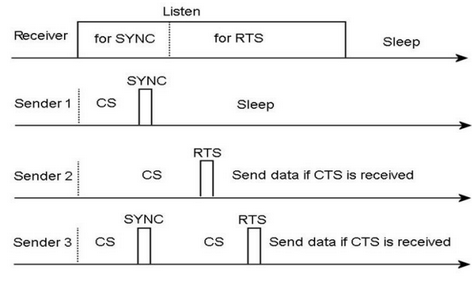
\includegraphics[width=0.7\linewidth]{images/smac-synchronization.png}
    \caption{S-MAC synchronization.}
    \label{fig:smac-synchronization}
\end{figure}

The process of sending SYNCs and coordinating them is often organized around minislots.
Think of the active period as subdivided into many tiny minislots (see Figure \ref{fig:smac-minislots}). A node that wants to transmit a SYNC will pick one minislot to check the channel and to end its carrier sense. If the channel looks free, the node transmits the SYNC in the following minislot. This randomized minislot selection spreads SYNC transmissions across different small time offsets, reducing the chance that multiple nodes’ SYNCs collide at the same instant.

\begin{figure}[ht]
    \centering
    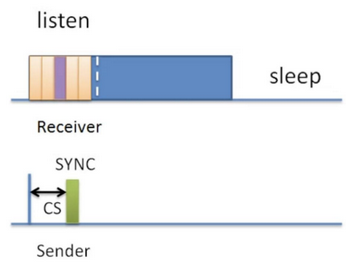
\includegraphics[width=0.4\linewidth]{images/smac-minislots.png}
    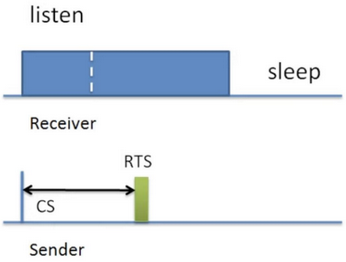
\includegraphics[width=0.39\linewidth]{images/smac-data-sending.png}
    \caption{S-MAC minislots \& data sending.}
    \label{fig:smac-minislots}
\end{figure}

S-MAC attacks the energy problem on several fronts:
\begin{itemize}
    \item \textit{Idle listening.} Turning the radio off during sleep windows dramatically cuts down this waste.
    \item \textit{Collisions} are mitigated with RTS/CTS for unicast exchanges, which reduces the need for costly retransmissions.
    \item \textit{Overhearing} is reduced because neighbors who hear an RTS or CTS not meant for them can sleep for the remaining duration.
\end{itemize}

Consider a small two-hop topology with two sources and two sinks (see Figure \ref{fig:smac-performance}). Each source periodically generates sensing messages that are split into fragments for transmission. The traffic load is varied by changing the inter-arrival period of messages: when the inter-arrival period is small (say 1 second) the traffic load is heavy because messages are generated frequently; when the inter-arrival period is large (say 10 seconds) the load is light.

\begin{figure}[ht]
    \centering
    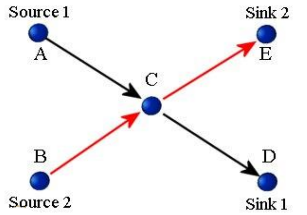
\includegraphics[width=0.4\linewidth]{images/smac-performance.png}
    \caption{SMAC performance evaluation.}
    \label{fig:smac-performance}
\end{figure}

For each test the experimenters fixed the total amount of data to be sent so they could compare energy usage per node for delivering the same workload. Specifically, each source generated 10 messages in the test; each message was divided into 10 fragments, and each fragment was 40 bytes. If you multiply that out you get the total packet count: two sources $\times$ 10 messages $\times$ 10 fragments equals 200 fragments (or data packets) that need to be delivered from sources to sinks. The experiment then measures the total energy each node consumes while sending that fixed amount of data under different traffic patterns.

The energy curves were then plotted against the message inter-arrival period (the time between new messages), so the horizontal axis is the inter-arrival period (smaller values mean heavier traffic), and the vertical axis is energy consumption in millijoules (see Figure \ref{fig:smac-experiment}).

\begin{figure}[ht]
    \centering
    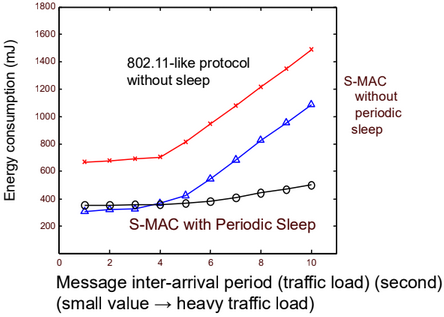
\includegraphics[width=0.6\linewidth]{images/smac-experiment.png}
    \caption{Average energy consumption in the source nodes A\&B.}
    \label{fig:smac-experiment}
\end{figure}

The plots compare three behaviors: an 802.11-like protocol without sleep, S-MAC without periodic sleep (which represents the S-MAC MAC behavior but with radios not sleeping), and S-MAC with periodic sleep. The key qualitative observations are:
\begin{itemize}
    \item When the traffic load is heavy (inter-arrival period small), idle listening becomes less important because radios are busy transmitting and receiving most of the time. In this regime the energy savings that come from sleeping are limited — everyone is active frequently and contention and transmission dominate energy costs. Thus the three curves converge and the advantage of periodic sleeping shrinks.
    \item When the traffic load is light (inter-arrival period large), nodes spend much of their time idle if they don’t sleep. That’s exactly when periodic sleeping shines. S-MAC with periodic sleep uses far less energy than the always-awake 802.11-like baseline because the radios are off most of the time and the node avoids idle listening and overhearing. The measured energy per node drops substantially as inter-arrival increases.
\end{itemize}
S-MAC assumes a mainly static network where nodes don’t move around much; schedules and neighbor tables are designed with that stability in mind. The protocol explicitly trades latency for energy: some transmissions must wait until receivers wake up, and border nodes may introduce extra delay because they juggle schedules.

Redundant data still flows, but it may flow with higher latency — S-MAC does not invent compression or deduplication; it optimizes when radios are on and off. Designers who need lower latency or higher throughput must either increase duty cycles or use other techniques (for example, reducing sleep intervals, using coordinated low-latency wakeups, or choosing a different MAC design).

\section{Routing}
\textit{Routing} is what lets sensor nodes pass data along from where it was sensed to the base station that collects it. Most realistic deployments use multi-hop communication: a packet may traverse several intermediate nodes before it reaches its destination. Because sensor nodes are usually battery powered, the routing strategy you choose has a huge effect on how long the network will live. Good routing finds paths that use as little energy as possible and balances load so a few nodes do not die early.

At a minimum, routing must reliably deliver packets from sensors to sinks. Beyond that, the questions that guide design are practical and energy-centered. Do you want a routing scheme where every node keeps a full picture of the network at all times, or one that only searches when it actually needs a route? Will node identities be arbitrary labels, or will you be able to use geographic position information? If nodes know their own locations, geographic routing becomes possible: you can pick the neighbor whose position is closest to the destination as the next hop, and that often reduces overhead because you don’t need global route tables.

Another high-level design choice is how to view network topology itself. If nodes are symmetric and play similar roles, you get a flat topology. If nodes are organized into clusters with cluster-heads you get a hierarchical topology.
When the network is flat, routing protocols for sensor networks fall into two major behavioral families, depending on when they operate.
\begin{itemize}
    \item \textit{Proactive} or \textit{table-driven} protocols always tries to keep routes up to date. Each node maintains routing entries for reachable destinations at all times. If you need to send a packet, the route is already in the table so there is no discovery delay. The price you pay is continuous overhead: periodic updates must be sent to keep tables fresh, and that consumes bandwidth and energy. Those updates also risk being out of date because wireless links change, so protocols include mechanisms to mark stale routes and correct inconsistencies.
    \item \textit{Reactive} or \textit{source-initiated}, on-demand protocols only discovers a route on demand. Route discovery happens only when an application actually needs to send data to some destination. That avoids the constant overhead of proactive approaches but it introduces latency up front: sending the first packet requires time to find a route. Reactive protocols sometimes keep a route cache, so if a recent route is still valid you get the best of both worlds—low overhead and low latency for cached destinations.
\end{itemize}
Some protocols blend the two behaviors into hybrids, choosing proactive behavior for nearby destinations and on-demand lookups for faraway ones.

\subsection{Destination Sequence Distance Vector (DSDV)}
A classic example of a proactive adaptation for ad hoc networks is \textit{Destination Sequence Distance Vector}, or DSDV. DSDV is a distance-vector protocol based on the distributed Bellman–Ford idea, but it adds sequence numbers and aging information to help prevent routing loops and to prefer fresh information.

DSDV periodically sends full routing updates. When topology changes, DSDV sends incremental updates that describe only the changes, reducing the volume of control traffic. If an update looks unstable the protocol may delay advertising the new route for a short time to avoid propagating transient, misleading information. That smoothing behavior reduces churn in the network state and lowers wasted transmissions.

Think of DSDV as everybody keeping a table that lists destinations, the next hop to reach each destination, and the cost (number of hops or other metric). In addition, each table entry carries a sequence number. A higher sequence number means the route information is more recent and therefore more trustworthy. When a node receives route updates from neighbors it prefers routes with larger sequence numbers. If two routes share the same sequence number, the one with the smaller cost (fewer hops) is chosen.

Sequence numbers solve a key problem of classic distance-vector algorithms: routing loops and count-to-infinity behaviors that can arise when nodes learn inconsistent information at different times. By tagging routes with sequence numbers and preferring fresh (higher-numbered) routes, DSDV converges toward loop-free behavior.

Let’s walk through a small example. Picture four nodes arranged in a row: Node \texttt{A} connects to \texttt{B}, \texttt{A} to \texttt{C}, and \texttt{C} to \texttt{D}. Initially every node knows only about itself and its immediate neighbors (see Figure \ref{fig:dsdv}). Each routing-table entry stores a destination, next hop, hop count, and a sequence number that increases when the destination originates new information.

Start with each node advertising itself with sequence number zero (or some base value) and cost zero. Neighboring nodes learn reachable destinations via their neighbors and build entries. Suppose \texttt{A} learns about \texttt{D} via \texttt{C} with a hop count of two; \texttt{B} learns about \texttt{D} via \texttt{A} and \texttt{D} with hop count of tree, and so on (see Figure \ref{fig:dsdv}).

\begin{figure}[ht]
    \centering
    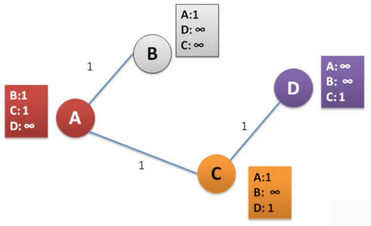
\includegraphics[height=0.27\linewidth]{images/dsdv.png}
    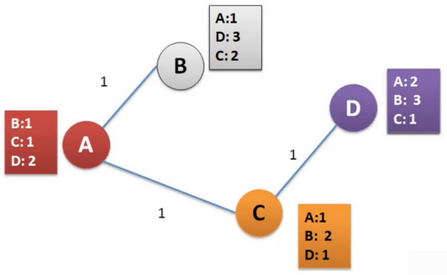
\includegraphics[height=0.27\linewidth]{images/dsdv-update.png}
    \caption{Destination Sequence Distance Vector example.}
    \label{fig:dsdv}
\end{figure}

Now imagine the link between \texttt{C} and \texttt{D} goes down. \texttt{C} detects the link failure and wants to inform everyone that \texttt{D} is unreachable through it. \texttt{C} increments the sequence number for \texttt{D} and advertises the route to D with an infinite metric (or a special flag) and the incremented sequence number. When \texttt{A} and \texttt{B} receive that update, they will see the larger sequence number and will mark that route as broken. They will then search for alternative routes—if none exist, they will also mark \texttt{D} unreachable.

If later \texttt{D} becomes reachable again via a different route (say \texttt{D} moves close to \texttt{B}), then \texttt{D} or \texttt{B} will advertise a new route to \texttt{D} with an even larger sequence number and an appropriate hop count. Because sequence numbers only increase, nodes will prefer the freshly advertised route over the older one and converge toward a consistent view without forming loops.

\subsection{Reactive Routing Protocols}
Reactive, or source-initiated, routing for wireless sensor networks is an on-demand way to find paths: instead of keeping a big routing table all the time, nodes look for routes only when they need them.

Reactive routing waits until some source node actually wants to send to a destination before it tries to find a path. When that moment comes, typically the source floods a route-request message into the network. Nodes forward the request while recording reverse-path information so replies can take the forward path back. When the request reaches the destination or an intermediate node that knows a fresh route to that destination, that node sends a route-reply back. The source then caches the discovered path and sends its data.

The disadvantage is initial latency and the cost of flooding control messages when discovering routes. Route caches can compensate for the delay problem. If a source has a recent, still-valid route in its cache, it can send immediately without discovery. 

\subsubsection{Flooding and Gossiping}
Two of the oldest reactive techniques are flooding and gossiping. They’re conceptually straightforward and help illustrate why more sophisticated reactive protocols exist.
\begin{itemize}
    \item \textit{Flooding} is exactly what it sounds like. A node that wants to send a packet broadcasts it to all neighbors. Each node that receives the packet forwards copies to all of its neighbors except the one it heard the packet from. Flooding tries every possible route automatically, so it has two nice properties: if any route exists between source and destination, flooding will find it; and one copy of the packet will travel along the fastest possible route, because flooding explores all routes in parallel.

    Those benefits come at a terrible cost. Flooding generates an enormous amount of redundant traffic. Nodes may receive many duplicate copies of the same message and forward them, producing implosion: neighbors repeatedly rebroadcast identical messages to the same nodes. If two sensors monitor the same event region, they might both send the same stimulus data at the same time and create overlap—redundant sensing that multiplies forwarding load. Worse, flooding is resource-blind: it doesn’t care how much battery each node has. Every node in the broadcast domain receives and forwards the packet, draining energy and shortening network lifetime.

    \item \textit{Gossiping} is a lower-chaos alternative. Instead of forwarding a packet to all neighbors, a node forwards it to a single randomly chosen neighbor (or to a small random subset). This avoids implosion because you typically keep just one copy of the message per node, but the tradeoff is slower spread: reaching every node in the network takes more hops and more rounds of random forwarding. Gossiping reduces redundancy and conserves energy compared to blind flooding, but it’s not ideal if you require fast, deterministic delivery to a specific destination.
\end{itemize}

\subsubsection{Dynamic Source Routing (DSR)}
\textit{Dynamic Source Routing (DSR)} is a clean, elegant reactive protocol that uses source routing. In source routing the sender places the full ordered list of hops that the packet should follow inside the packet header. That header tells every forwarding node exactly where to send the packet next; no per-node routing table lookups are needed for forwarding.

DSR has two core mechanisms that work on demand. 
\begin{itemize}
    \item \textit{Route discovery} is invoked when a node has a packet for some destination but no suitable route in its cache. 
    \item \textit{Route maintenance} watches the paths currently in use and notifies the sender if a link along a source route breaks.
\end{itemize}
Here’s how route discovery works, step by step, in the classic RFC example. Imagine node \texttt{A} wants to reach node \texttt{E} but doesn’t have a route cached. \texttt{A} broadcasts a Route Request (RREQ). The RREQ contains three critical pieces of information: the identity of the initiator (\texttt{A}), the identity of the target (\texttt{E}), and a unique request identifier. It also contains a route record that starts as an empty list (or as \texttt{[A]} if you consider \texttt{A} listed).

Each node that receives the RREQ appends its own address to the route record and rebroadcasts the request, unless it has already seen this RREQ identifier (in which case it discards the duplicate). Over time the route record accumulates the sequence of nodes the RREQ has traversed: first \texttt{A}, then \texttt{A},\texttt{B}, then \texttt{A},\texttt{B},\texttt{C}, then \texttt{A},\texttt{B},\texttt{C},\texttt{D}, and finally the request reaches \texttt{E} with the record \texttt{[A,B,C,D]}.

When the target \texttt{E} receives the RREQ, it can construct a Route Reply (RREP) containing the complete reverse route. If source routing is used in the reply, the RREP will list the route \texttt{E},\texttt{D},\texttt{C},\texttt{B},\texttt{A} or simply use the accumulated record reversed. The initiator receives the RREP, caches the discovered source route, and starts sending data with that source route included in each packet header.

A few practical niceties follow from this mechanism. First, because the source route is in the packet header, any node that overhears packets can cache the route for future reuse. Second, a single route discovery may discover multiple distinct routes because different RREQ copies can reach the destination via different paths; the initiator can cache several alternatives to react quickly to failures. Third, when a link on a cached route breaks during data forwarding, the sender is informed (often by an explicit route-error message generated by the detecting node), and the sender can try another cached route before initiating a new global discovery.

\begin{Example}{Route discovery}{}
To make this concrete, visualize a small network of nodes labeled 1 through 7. Node 1 broadcasts a route request for node 5. As the request spreads it may arrive at different neighbors with different accumulated route records: one copy might arrive at a node as [1,4], another as [1,7], another as [1,7,3], and so on, depending on which path the RREQ took. When node 5 finally receives one of these copies, it sends back a reply that includes the accumulated record—say it replies with [5,3,7,1], which reversed yields the forward path 1$\to$ 7$\to$3$\to$ 5. That route is cached and immediately usable. Because multiple RREQs can reach 5 through different paths, node 1 can learn multiple distinct routes from a single discovery event.

\begin{minipage}{\textwidth}
    \centering
    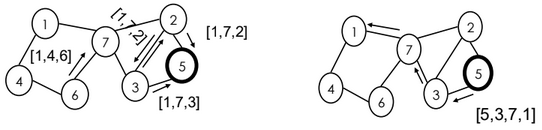
\includegraphics[width=0.8\linewidth]{images/route-discovery.png}
    %\captionsetup{hypcap=false}
    %\captionof{figure}{Query tree.}
    \label{fig:route-discovery}
\end{minipage}
\end{Example}

Route maintenance detects when a link in a source route stops working. For example, if node X forwards a packet but does not hear the expected link-layer acknowledgment, X can generate a route-error and send it back to the source. The source then removes any cached routes that use the broken link and either tries another cached route or launches a fresh route discovery.

Because DSR supports caching multiple routes to a single destination, recovery is often quick: a failed route can be swapped out for a backup route without immediate global flooding.

\subsubsection{Ad hoc On-Demand Distance Vector (AODV)}
\textit{Ad hoc On Demand Distance Vector (AODV)} takes much of the discovery spirit of DSR but avoids source routing and the large per-packet header overhead by using routing tables at intermediate nodes. AODV is widely used in ad hoc networking and is a natural reactive complement to DSR.

When a source needs a route and has none in its table, it broadcasts a Route Request (RREQ). Intermediate nodes forward the RREQ, and while doing so they record a reverse path toward the source: the first neighbor from which the RREQ came is recorded as the next hop toward the source. When the RREQ reaches the destination (or an intermediate node that knows a fresh route), that node unicasts a Route Reply (RREP) back along the reverse path. As the RREP is forwarded back to the source, intermediate nodes install forward route entries pointing to the neighbor from which the RREP was received. After the process completes, the source and the intermediate nodes along the path all have routing-table entries enabling future unicast forwarding without carrying the full path in packet headers.

AODV also uses sequence numbers to ensure freshness and avoid routing loops. Each route entry is tagged with a destination sequence number, and nodes only adopt routes with newer (larger) sequence numbers, similar in spirit to DSDV. Sequence numbers help nodes decide whether an intermediate node’s cached route is fresh enough to be used when responding to a RREQ.

The learning of reverse and forward paths is a neat, efficient side effect: the RREQ sets up the reverse path, while the RREP establishes the forward path. If a link fails, AODV supports local repair or route error messages that notify affected upstream nodes, which then invalidate stale entries and may trigger new route discoveries.

\begin{Example}{AODV}{}
Let's walk through an example discovery from the point of view of one source \texttt{S} wanting to talk to destination \texttt{D}.

\begin{minipage}{\textwidth}
    \centering
    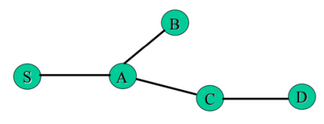
\includegraphics[width=0.6\linewidth]{images/aodv-example.png}
    %\captionsetup{hypcap=false}
    %\captionof{figure}{Query tree.}
    \label{fig:aodv-example}
\end{minipage}

Source \texttt{S} has a packet for \texttt{D} but no route in its table. \texttt{S} broadcasts a Route Request (RREQ). The RREQ contains the identities of \texttt{S} and \texttt{D}, a unique request identifier, and other control fields such as sequence numbers that help judge route freshness.

When a neighbor (call it \texttt{A}) receives \texttt{S}’s RREQ it stores a reverse route entry toward \texttt{S} in its routing table: “To reach \texttt{S}, next hop is \texttt{S}.” That reverse entry is used later to deliver replies back to the source. Then \texttt{A} rebroadcasts the RREQ to its neighbors.

The next node (call it \texttt{C}) that receives \texttt{A}’s rebroadcast records a reverse route toward \texttt{S} as well. In \texttt{C}’s table you now have “To reach \texttt{S}, next hop is \texttt{A}.” \texttt{C} then rebroadcasts the RREQ onward.

At some point the RREQ reaches a node that can answer. This might be the destination \texttt{D} itself or some intermediate node that already has a fresh route to \texttt{D}. Suppose node \texttt{C} is such a node and decides it can answer. \texttt{C} creates a Route Reply (RREP) and unicasts it back toward \texttt{S} using the reverse path already recorded.

As the RREP travels back along the reverse path (for example \texttt{C} $\to$ \texttt{A} $\to$ \texttt{S}), each intermediate node installs a forward route toward \texttt{D}. Concretely, when \texttt{A} receives the RREP from \texttt{C} it records “To reach \texttt{D}, next hop is \texttt{C}.” Inserting these forward entries prepares intermediate nodes to forward subsequent data packets without requiring source routing.

Finally the RREP reaches the originator \texttt{S}. \texttt{S} installs a route entry “To reach \texttt{D}, next hop is \texttt{A}” (assuming \texttt{A} is the neighbor on the reverse path) and can immediately start sending data along the newly discovered path \texttt{S} $\to$ \texttt{A} $\to$ C $\to$ ... $\to$ \texttt{D}.
\end{Example}


\subsection{Geographic routing}
Traditional routing expects each node to keep a table that maps destinations to next hops. An alternative, which is very natural for sensor networks, is to infer forwarding decisions implicitly from the physical placement of nodes. If every node knows its own position, knows the positions of its immediate neighbors, and knows the destination’s location, the node can choose a neighbor that moves the packet closer to the destination.

This family of ideas is called \textit{geographic routing} or position-based routing. It’s especially appealing in large sensor deployments because you avoid the global state and periodic updates required by full routing tables. Two related concepts are worth naming: \textit{geocasting}, which is “send a packet to any node in a given geographic area,” and \textit{position-assisted routing} more generally, where a location service may be used to map a node ID to a geographic coordinate when the node’s exact location is needed.

The most common greedy strategy is called \textit{“most forward within range r”}. Imagine you are node \texttt{S} and you want to forward a packet toward destination \texttt{D}. Look at all neighbors within your communication range (distance $\leq r$) and pick the neighbor that makes the most forward progress toward \texttt{D}. Concretely, that means pick the neighbor for which the remaining distance to \texttt{D} becomes smallest after the hop (see Figure \ref{fig:position-based-routing}).

\begin{figure}
    \centering
    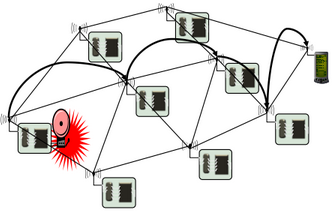
\includegraphics[width=0.5\linewidth]{images/position-based-routing.png}
    \caption{Position based routing: most forward within range $r$.}
    \label{fig:position-based-routing}
\end{figure}

One important clarification: “most forward progress” is not the same as “farthest from the sender.” A neighbor that is far from \texttt{S} but sideways relative to the S$\to$ \texttt{D} line may not reduce the remaining distance to \texttt{D} at all. You want the neighbor that reduces the remaining distance to the destination most, not the one that simply maximizes hop length.

Greedy is the classic baseline, but designers often tweak it to meet other goals:
\begin{itemize}
    \item choose the nearest neighbor that still makes forward progress. The idea here is to minimize transmit power: short hops consume less power per transmission even though they may increase hop count. If radios support power control, taking a close neighbor that still moves the packet forward can save energy.
    \item directional or angular routing. Instead of comparing distances, pick the neighbor whose bearing is closest to the bearing of the destination (angular closeness). Or pick the neighbor whose projection onto the straight line from \texttt{S} to \texttt{D} is closest (minimize perpendicular distance). These ideas try to keep the packet moving along a straight path, but they can accidentally form loops if the geometry and neighbor set interact poorly.
\end{itemize}
Greedy forwarding can fail. A packet can arrive at a node that has no neighbor closer to the destination than itself. That situation is called a \textit{dead end} or local minimum (see Figure \ref{fig:dead-ends}). When greedy forwarding hits a dead end, you need a fallback strategy.

\begin{figure}[ht]
    \centering
    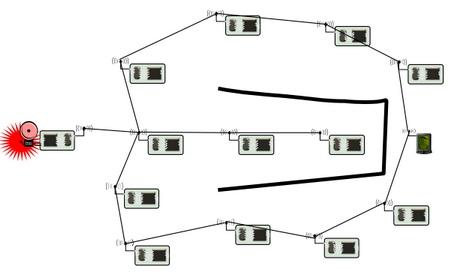
\includegraphics[width=0.6\linewidth]{images/dead-ends.png}
    \caption{Dead ends.}
    \label{fig:dead-ends}
\end{figure}

When nodes know positions, routing can be dramatically simpler and more scalable. Position-based techniques avoid the overhead of maintaining global route tables and they scale nicely: each node only needs neighbor coordinates (local information) and possibly a lightweight location service when destination coordinates aren’t known locally.

Which approach is best still depends on network characteristics: mobility, node capabilities (do they have GPS? can they measure signal strength?), application traffic patterns, energy budgets, and so on. For highly mobile networks (drones, vehicles), position-based methods can help because they avoid stale global tables and position-based routing uses local neighbor information that changes locally and can be updated cheaply.
